% Target: 35 pages
% Current: 3

\chapter{Adapters Effectiveness in Machine Translation}
\label{chap:adaptefct}
In this chapter, we continue the study from the previous chapter to understand more about the relation between adapters and pre-trained models. Like the previous chapter, we use BERT and its variance as the base pre-trained models and fine-tune them with adapters. The difference with the previous chapter is that we do not use our pre-trained language models and focus solely on the BERT weights. This study evaluates the combination of adapters and transformer models on machine translation tasks and studies adapters' effectiveness by putting them only in the encoder or the decoder. We evaluate the models on the machine translation task. We also experiment with down-scaling the pre-trained model size and try to recover the performance from being comparable to the full-sized model. We conduct the experiments by separating them into three different areas:
\begin{itemize}
    \item Use BERT weights\footnote{We use publicly available BERT weights from Huggingface hub \url{https://huggingface.co}} as the pre-train weights and investigate the importance of adapters in encoder or decoder.
    \item Use BERT weights and investigate their importance compared to random weights in the encoder or decoder while fine-tuning with adapters.
    \item Down-scaling BERT weights by either zeroing out half of BERT's weights (\texttt{zbert}) or completely removing them from the weight matrices, squashing the matrices (\texttt{zsbert}). We use the down-scaling technique to understand whether we can use adapters to recover the performance of the original BERT (without adapters) while using fewer parameters.
\end{itemize}

\section{Fixed Variable Parameters of Experients}
\subsection{Framework}
\begin{table}[]
    \centering
    \begin{tabular}{@{}cc@{}}
        \toprule
        \textbf{Name}            & \textbf{Value}        \\ \midrule
        \textbf{Batch size}      & 64                    \\
        \textbf{Learning rate}   & 0.0005                \\
        \textbf{Vocabulary size} & 31102 (de), 30522(en) \\ \bottomrule
    \end{tabular}
    \caption{Fixed hyperparameters throughout the experiments}
    \label{tab:hyp_invest}
\end{table}

As we mentioned at the beginning of the chapter, we have several scenarios we use to conduct the experiments. Despite various possibilities of different setups, we now describe variables that we fixed throughout the experiments. As mentioned in Chapter \cref{chap:03}, we use Huggingface as our main framework with added modifications for adapters. In contrary to Chapter \ref{chap:adaptmt}, we do not investigate language models that we train ourselves, but instead, we focus mainly on the BERT language model. We use the same hyperparameters to Chapter \ref{chap:03} which we describe on \cref{tab:hyp_invest}.

The model and hyperparameters that we use throughout the experiment remain the same as described in Chapter \ref{chap:adaptmt}. We use transformer model with seq2seq architecture, and we follow BERT-based configuration to initialize both the encoder and the decoder.

\subsection{Dataset}
As mentioned in the previous section, we focus mainly on machine translation tasks. We have already described in Chapter \ref{chap:03} that WMT is mainly used for language model training and mixed training for models that were trained from scratch. For machine translation, we focus solely on IWSLT to fine-tune and evaluate our models.

\section{Original BERT}
\subsection{Size of Adapters}
\subsubsection{Experiment Setup and Motivation}
\paragraph{}
In these experiments, we keep the weights of the transformer model intact and only modify the reduction ratio parameter in the adapters. Adapters serve as bottleneck layers that reduce the input size dimension before scaling it back. The reduction ratio is defined as the number of dimensions that we reduce within the bottleneck layer. To be more precise, if we use ``16'' as the reduction ratio, we reduce the original layers by ``16'' and then scale it back to the original size.

We are using various sizes of reduction ratios to compare the result. This reduction aims to see whether we can further benefit from enlarging the adapters' bottleneck size in terms of performance. We use 16, 8, 4, 2, and 1 as the ratio values for this experiment. We compare the results with the baseline BERT that we fine-tuned by only modifying the cross-attention layer. We will refer to this baseline as baseline BERT for the entirety of this work.

\subsubsection{Experiment Results}
In this section, we compare the results of the baseline BERT (only cross-attention fine-tuned) with fine-tuned models with adapters in different reduction ratios. We only fine-tuned the cross-attention layers for the baseline BERT model and kept the rest of the weights intact. We can see in \cref{img:adapt_bert_ratio} that even the smallest model (\texttt{adapt\_bert\_reduc\_16}) can already outperform the baseline by around 2 BLEU. This shows that the adapters can help improve the model's performance by adding only a small number of weights during the fine-tuning.

\begin{figure}[]
    {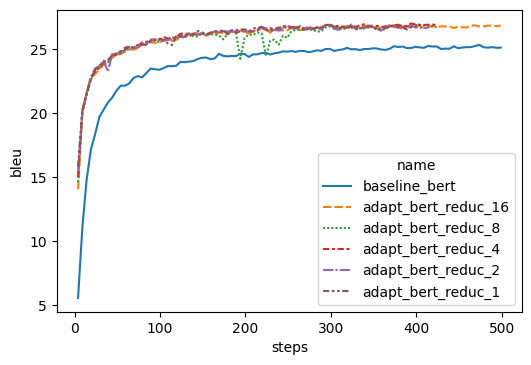
\includegraphics[width=0.95\textwidth]{img/adapter_bert_baseline_adapters.png}}
    \centering
    \caption{Comparison between baseline BERT model and adapters model with different ratio (16, 8, 4, 2, 1).}
    \label{img:adapt_bert_ratio}
\end{figure}

Furthermore, the difference between the ratios is minimal. It suggests that there is not much benefit in expanding the size of adapters for the normal size BERT. It is possible that it is no longer trivial to append adapters to fine-tune the model for large-sized models such as the original BERT. Further changes may be required to handle the different nature of BERT's output as it is naturally different from the common auto-regressive machine translation objective.

\subsection{Position of Adapters (Encoder vs Decoder)}
\label{sec:posada}
\subsubsection{Experiment Setup and Motivation}
We would like to see the importance of adapters when they are put in different places. Since we are working with seq2seq architecture in this work, we would like to see whether only incorporating adapters on one side can already be beneficial and reduce the weight added to the model.

\subsubsection{Experiment Result}
\begin{figure}[]
    {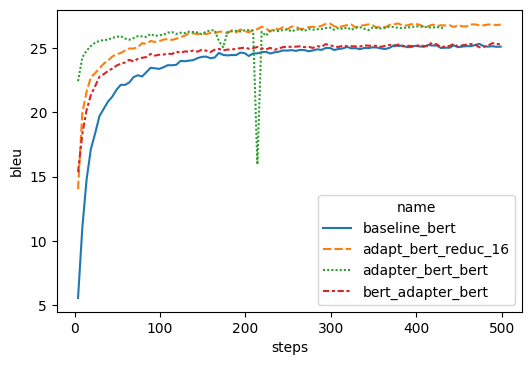
\includegraphics[width=0.95\textwidth]{img/bert_pos.png}}
    \centering
    \caption[Results of ablation study for adapters in the encoder or the decoder.]{Comparison between baseline BERT model and adapters model where the adapters are placed in three different setups: 1) Adapters in both encoder and decoder (\texttt{adapt\_bert\_reduc\_16}); 2) Adapters only in encoder (\texttt{adapter\_bert\_bert}); 3) Adapters only in decoder (\texttt{bert\_adapter\_bert}).}
    \label{img:adapt_bert_pos}
\end{figure}
We see in \cref{img:adapt_bert_pos} that adding adapters just in the encoder part brings an improvement and outperforms the baseline. Adapters only in the encoder train the fastest at the beginning, and their final performance is almost the same as if we added the adapters on both sides. For the decoder, on the other hand, we can see that aside from a more promising start, there is no benefit as there is no improvement in terms of late BLEU scores compared to the baseline. With this finding, we can reduce the cost of fine-tuning further by half when we do not include the adapters on the decoder.
% Adding the adapters on the encoder and fine-tuning it is more cost-effective than the decoder. With this finding, we can reduce the cost of fine-tuning by half when we do not include the adapters on the decoder.

\subsection{True BERT in Encoder vs Decoder}
\label{sec:pospre}
\subsubsection{Experiment Setup and Motivation}
This section investigates the importance of having BERT the pre-training models as the initial weights in either the encoder or decoder. In addition to that, we also expand the experiment further by understanding the correlation of adding adapters on top of the randomly set weights.

We start by describing the setup in this experiment. The previous chapter introduced an experiment where we instantiate the base transformer model with only random weights. We then fine-tune the base transformer model by only updating the adapters and cross-attention layer. In this setup, we are doing experiments in a similar concept. We use random (fixed) weights instead of the original pre-trained BERT weights. We thus have a seq2seq model with the random weights encoder followed by the BERT decoder and vice versa. In the fine-tuning stage, we update both the adapters in the encoder and decoder and the cross-attention layer (or cross-attention layer only in our baseline models).

The purpose of the experiments are:
\begin{itemize}
    \item We want to understand further the importance of the pre-training model when fine-tuned with adapters. By initializing the model with BERT only in one component, we can see whether it is necessary to use BERT on both components when adapters are incorporated.
    \item We want to understand the capability of adapters when either one of the components does not contain useful information (relative to BERT). We would like to see whether the adapters can recover or even outperform some of the performance that we have already gathered from the previous chapters and sections.
\end{itemize}

\subsubsection{Experiment Results}
This section compares models that use adapters in either or both the encoder and decoder while only initializing one of these components with true BERT weights and the other one with (fixed) random weights. The purpose of the experiments is to understand the behaviour of adapters when faced with relatively poor representation in one of the components.

\paragraph{Randomly Set Weights on Encoder}
In this part of the section, we want to answer the main question: "To what extent can the adapters restore the missing gap when the encoder does not contain useful information (relative to BERT)?"

\begin{figure}[h]
    {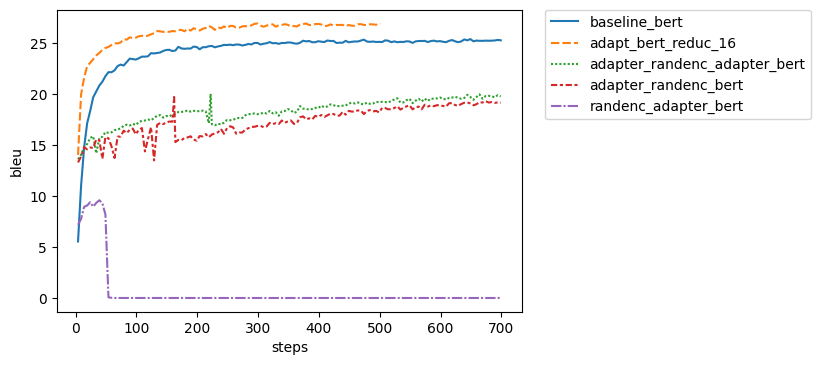
\includegraphics[width=0.95\textwidth]{img/adapter_bert_randenc.png}}
    \centering
    \caption[Comparison for model with adapters in the decoder and the encoder is initalized with random weights.]{Comparison between baseline BERT model and adapters model where the adapters are placed in three different setups: 1) Adapters in both encoder and decoder (\texttt{adapt\_bert\_reduc\_16}); 2) Adapters only in encoder (\texttt{adapter\_bert\_bert}); 3) Adapters only in decoder (\texttt{bert\_adapter\_bert}) and the decoder is initialized with BERT while the encoder is initialized with random numbers.}
    \label{img:adapt_bert_randenc}
\end{figure}

We can see from \cref{img:adapt_bert_randenc} that when adapters are appended in both components, we get to almost 20 in the BLEU score. This is relatively higher than the other two setups (adapters only in the encoder and only in the decoder). However, compared to the baseline, we are missing 4 points in BLEU when we set the weights on the encoder as entirely random. This means that the base encoder model was missing relatively essential information that the adapters can not simply restore during the fine-tuning.

We further focus on the adapters' performance compared to the baseline model that is only fine-tuned on the cross-attention layer to see whether there is any benefit in using adapters or simply fine-tuning the cross-attention already enough. We can see that the model that was only fine-tuning the cross-attention layer can not learn at all, while the adapters can perform significantly better. This marks the capability of the adapter when faced with a randomly set encoder.

When the adapters are removed from the decoder, we see a degradation in performance in about 1 BLEU. However, when the adapters are removed from the encoder, we can see the performance is completely depleted during the training. We also see the same behaviour in the next section when the weights on the decoder are set randomly. This tells us that there is some incompatibility in the weights (random and BERT) where it is not trivial to fine-tune the cross-attention layer without further adjustment to the base model's weights.

\paragraph{Randomly Set Weights on Decoder}
Similar to the previous section, the main question in this experiment is, "To what extent can the adapters restore the missing gap when the decoder does not contain useful information (relative to BERT)?"

In contrast to when the randomly set weights are on the encoder side, we can see from \cref{img:adapt_bert_randdec} that the model has comparable performance to the one we have on the BERT baseline. This tells us that the pre-training weights in the encoder are more critical than in the decoder when we have adapters on both sides. However, when removing the adapters on the encoder side, we see similar performance as in the previous section, where the performance drops to zero in the middle of training. This further strengthens our arguments that adapters are necessary to adjust the weights in the model so that the cross-attention layer can work properly.

\begin{figure}[h]
    {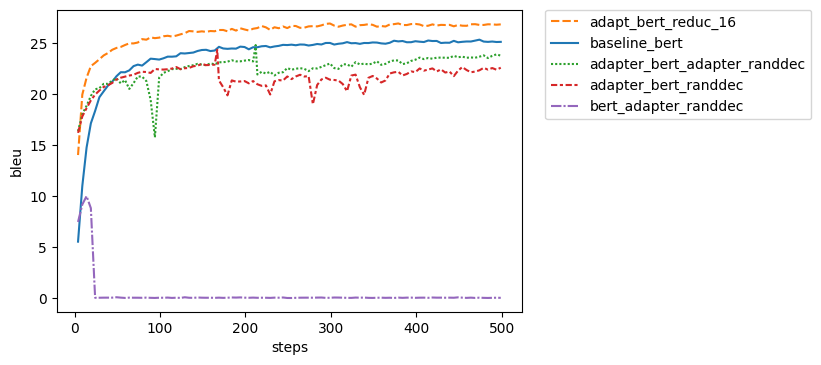
\includegraphics[width=0.95\textwidth]{img/adapter_bert_randdec.png}}
    \centering
    \caption[Comparison for model with adapters in the decoder and the decoder is initalized with random weights]{Comparison between baseline BERT model and adapters model where the adapters are placed in three different setups: 1) Adapters in both encoder and decoder (\texttt{adapt\_bert\_reduc\_16}); 2) Adapters only in encoder (\texttt{adapter\_bert\_bert}); 3) Adapters only in decoder (\texttt{bert\_adapter\_bert}) and the encoder is initialized with BERT while the decoder is initialized with random numbers.}
    \label{img:adapt_bert_randdec}
\end{figure}

On the other hand, when we remove the adapters from the decoder side, we can see that the performance is not as bad as when the adapters are removed from the encoder, but we still see a reduction in performance. We see around $<$ 1 BLEU when the model reaches 400k steps in the training stage.

\section{BERT Size Reduction}
\subsection{Zeroing Columns}
\subsubsection{Experiment Setup and Motivation}
In this experiment, we will focus on the soft reduction of BERT weights by zeroing the weights on every even index column and row in both the transformer body as well as in the embedding weights. We load pre-trained BERT weights, manually edit them and then continue the experiments by fine-tuning the cross-attention and adapters. We further refer to this setup as \texttt{zbert} for the rest of this writing.

Besides removing the columns, we also perform experiments where we put the adapters either on the encoder or the decoder. The goal of this particular experiment is to understand the behaviour of the model when the pre-trained models are replaced with this particular setup.

\subsubsection{Comparison with BERT Baseline (Full BERT Fine-tuning)}
We first compare the \texttt{zbert} model without adapters and only fine-tuning the cross-attention layers. We use \texttt{zbert} weights on both encoder and decoder so that it is comparable to the model that uses full-weight BERT. We use the full-weight BERT as the baseline in this experiment.

\begin{figure}[]
    {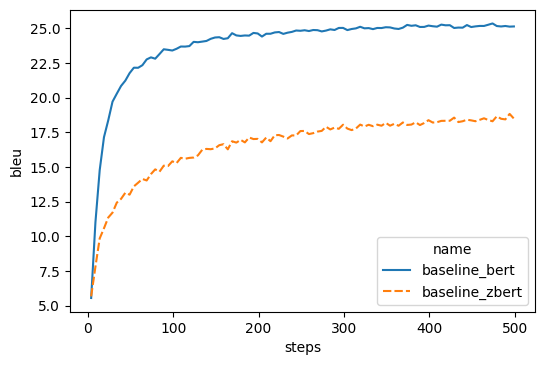
\includegraphics[width=0.95\textwidth]{img/baseline_zbert.png}}
    \centering
    \caption{Comparison between baseline BERT model and baseline \texttt{zbert} models.}
    \label{img:baseline_zbert}
\end{figure}

\begin{figure}[]
    {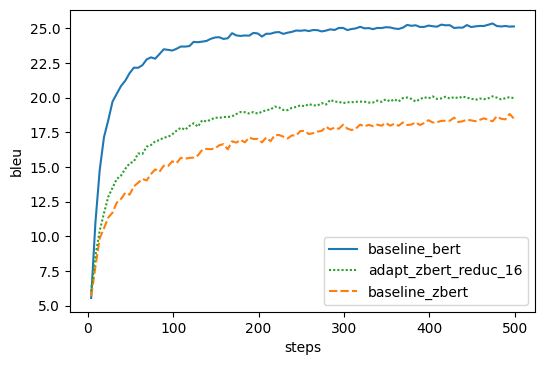
\includegraphics[width=0.95\textwidth]{img/adapter_zbert.png}}
    \centering
    \caption{Comparison between baseline BERT model, baseline \texttt{zbert} and adapters \texttt{zbert} models.}
    \label{img:adapter_zbert}
\end{figure}

We can see in \cref{img:baseline_zbert} that we are losing performance of about 4 BLEU. This is significant as we are losing various essential features from the original BERT model. To see whether we can recover some of the performance with adapters, we continue our experiment by fine-tuning \texttt{zbert} model that is instantiated on both encoder and decoder sides with adapters. We can see from \cref{img:adapter_zbert} that we only managed to recover 1 BLEU with a reduction ratio of 16.

\begin{figure}[]
    {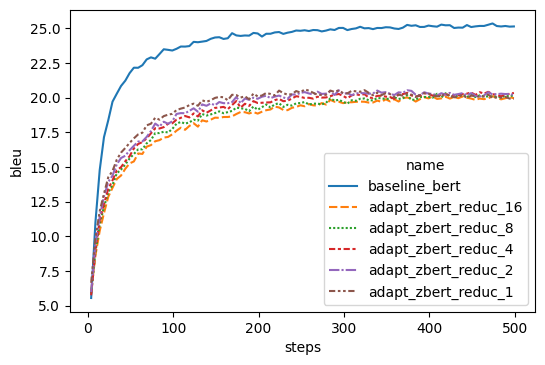
\includegraphics[width=0.95\textwidth]{img/adapter_zbert_ratio.png}}
    \centering
    \caption{Comparison between baseline BERT model and different reduction ratio of \texttt{zbert} models.}
    \label{img:adapter_zbert_ratio}
\end{figure}

From \cref{img:adapter_zbert_ratio}, when we increase the size of the reduction ratio, initially, we can see some improvement in the BLEU score compared to the higher ratio. However, they eventually converge to a similar performance by the end of training with no significant difference between different ratios. From this result, we can understand that depending on the base pre-trained model, adapters still have a limitation in achieving certain performance.

\paragraph{Adapters Position}
In this section, we aim to understand whether the position of both adapters and the pre-training models affect the model performance, similar to what we have seen in \cref{sec:posada}. We use a similar setup as in the previous section, with the exception that we use \texttt{zbert} as the pre-trained model instead of the original BERT model.

\begin{figure}[h]
    {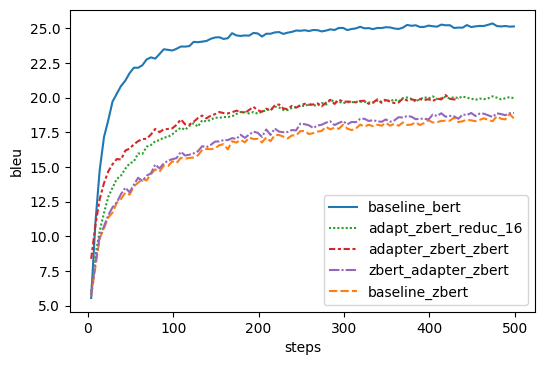
\includegraphics[width=0.95\textwidth]{img/zbert_pos.png}}
    \centering
    \caption[Comparison between baseline BERT and \texttt{zbert} models.]{Comparison between baseline BERT model, baseline \texttt{zbert} model, adapters in both encoder and decoder of \texttt{zbert} model (\texttt{adapt\_zbert\_reduc\_16}), adapters only in encoder of \texttt{zbert} model (\texttt{adapter\_zbert\_zbert}), and adapters only in decoder of \texttt{zbert} model (\texttt{zbert\_adapter\_zbert}).}
    \label{img:zbert_pos}
\end{figure}

We can see from \cref{img:zbert_pos} that when we include adapters on both encoder and decoder, we can outperform the baseline \texttt{zbert} in around 2 BLEU points. This shows that similar to the models that use BERT as the pre-trained models, the adapters can help to improve the performance further even though some of the information is already missing in the base model.

Furthermore, we can also see that similar to the BERT model that was fine-tuned with adapters, using adapters only on the encoder side performs much better than on the decoder side. Other than that, we can also see that incorporating adapters only on the encoder side helps the model achieve better performance faster than the model that uses adapters on both sides. This further support our hypothesis that updating the representation on the encoder side is more beneficial. Looking deeper at the model with adapters only on the decoder, the performance is close to the baseline model, where we only fine-tune the cross-attention layer. This could mean that fine-tuning the decoder may not be enough to achieve better performance when the representation from the source side is constant.

\subsection{Model Down-scaling}
\subsubsection{Experiment Setup and Motivation}
This experiment is the follow-up from \texttt{zbert} where we zeroed out half of the elements in the matrices. To be more specific, we are now completely removing those elements from the matrix instead of just zeroing out the elements. The way we do this is similar to the one we do on \texttt{zsbert}. We remove the matrix elements on every even column and row in both the transformer body as well as the embedding weights. We similarly do the weights processing offline before using it as the pre-training base model. For the rest of this writing, we refer to this setup as \texttt{zsbert}.

Furthermore, we also follow a similar setup as in \cref{sec:posada} where we experiment with the position of the adapters. The goal of this experiment is that we would like to understand the behaviour of the model compared to the baseline as well as \texttt{zbert}.

\subsubsection{Comparison with BERT Baseline and \texttt{zbert}}

\begin{figure}[h]
    {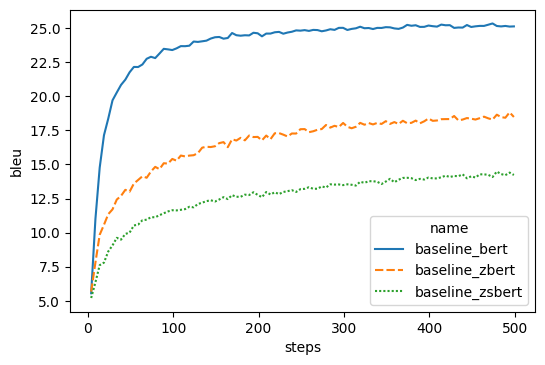
\includegraphics[width=0.95\textwidth]{img/baseline_zsbert.png}}
    \centering
    \caption{Comparison between baseline BERT model and baseline \texttt{zsbert} model.}
    \label{img:baseline_zsbert}
\end{figure}

\begin{figure}[]
    {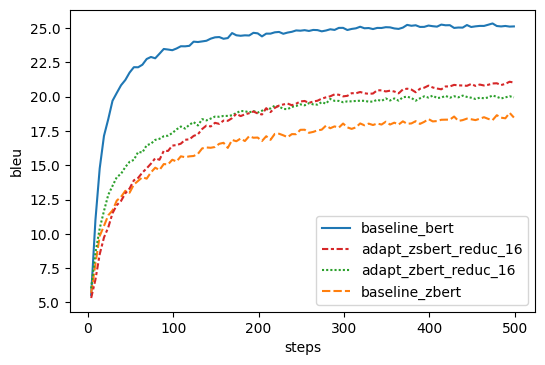
\includegraphics[width=0.95\textwidth]{img/adapter_zsbert.png}}
    \centering
    \caption{Comparison between baseline BERT model, baseline \texttt{zbert}, baseline \texttt{zsbert} and adapters \texttt{zsbert} models.}
    \label{img:adapter_zsbert}
\end{figure}


We begin with the comparison of \texttt{zsbert} with the BERT baseline. We see in \cref{img:baseline_zsbert} that the performance degrades by almost 10 BLEU points. This is also significantly worse than \texttt{zbert} where we only lose 5 BLEU. After some investigation, we realized that removing weights from the network is not straightforward as the computation of layer normalization depends on the matrix size and the adapter scaling factor will also be different. With manual evaluation, we found a slight difference between the only zeroed weights and the completely removed weights. This slight difference in the output of layer normalization gets propagated to the top layers, causing the result to differ significantly.

% Next, we study the interplay of model down-scaling and adapters. We can see in \cref{img:adapter_zsbert} that adapters with a 16 ratio manage to improve the performance up to 6 BLEU compared to \texttt{zbert} without adapters.
% We also notice a leap in final performance when we compare the adapter model with an equal reduction ratio (16) between \texttt{zbert} and \texttt{zsbert}. We can see that initially \texttt{zsbert} performs worse than \texttt{zbert}. After some steps, we can see the performance in \texttt{zbert} starting to stall but not in \texttt{zsbert}. We hypothesize that this relates to a similar reason that we stated in the original BERT model, where we could not see any improvement when increasing the reduction ratio. It is possible that when we reduce the size of the original pre-trained model, the adapters manage to adjust the flow of information within the network and better replace the missing information with new knowledge that is more important for solving the task.

\begin{figure}[]
    {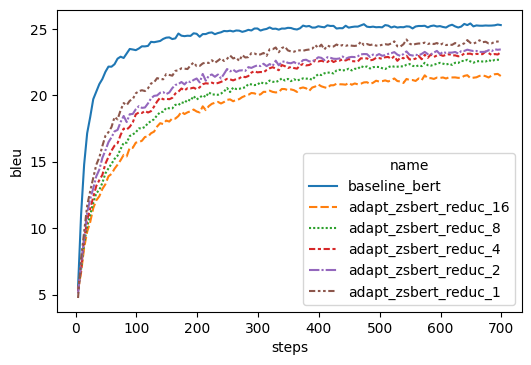
\includegraphics[width=0.95\textwidth]{img/adapter_zsbert_ratio.png}}
    \centering
    \caption{Comparison between baseline BERT model and different reduction ratio of \texttt{zsbert} models.}
    \label{img:adapter_zsbert_ratio}
\end{figure}

In \cref{img:adapter_zsbert_ratio}, when the adapters reduction ratio is further reduced, we can see that the performance is also improving up to the point where it has close performance to the baseline model. This remarks a prominent result as we can see from \cref{tab:numvars} that the total number of weights (including adapters) is reduced significantly.

\begin{table*}[]
    \centering
    \begin{tabular}{@{}cccc@{}}
        \toprule
        \textbf{Name}                                                               &
        \textbf{\begin{tabular}[c]{@{}c@{}}\# Trainable\\ Variables\end{tabular}}   &
        \textbf{\begin{tabular}[c]{@{}c@{}}\# Untrainable\\ Variables\end{tabular}} &
        \textbf{\begin{tabular}[c]{@{}c@{}}\# Total\\ Variables\end{tabular}}                                                \\ \midrule
        \textbf{Adapters ratio 16}                                                  & 7.736.826  & 95.143.296  & 102.880.122 \\
        \textbf{Adapters ratio 8}                                                   & 8.179.770  & 95.143.296  & 103.323.066 \\
        \textbf{Adapters ratio 4}                                                   & 9.065.658  & 95.143.296  & 104.208.954 \\
        \textbf{Adapters ratio 2}                                                   & 10.837.434 & 95.143.296  & 105.980.730 \\
        \textbf{Adapters ratio 1}                                                   & 14.380.986 & 95.143.296  & 109.524.282 \\
        \textbf{Normal BERT}                                                        & 28.990.078 & 218.819.328 & 247.809.406 \\ \bottomrule
    \end{tabular}
    \caption{Total trainable variables in \texttt{zsbert} with adapters on different ratio vs normal BERT model}
    \label{tab:numvars}
\end{table*}

\subsubsection{Adapters Position}

\begin{figure}[h]
    {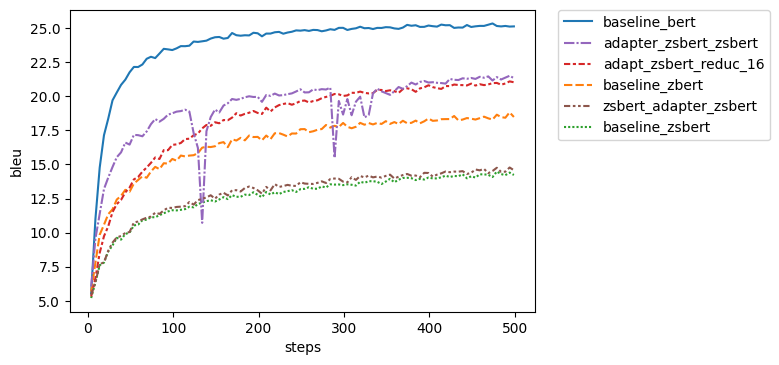
\includegraphics[width=0.95\textwidth]{img/zsbert_pos.png}}
    \centering
    \caption[Comparison between baseline BERT and \texttt{zsbert} models.]{Comparison between baseline BERT model, baseline \texttt{zsbert} model, adapters in both encoder and decoder of \texttt{zsbert} model (\texttt{adapt\_zsbert\_reduc\_16}), adapters only in encoder of \texttt{zsbert} model (\texttt{adapter\_zsbert\_zsbert}), and adapters only in decoder of \texttt{zsbert} model (\texttt{zsbert\_adapter\_zsbert}).}
    \label{img:zsbert_pos}
\end{figure}

From \cref{img:zsbert_pos}, similar to the \texttt{zbert} experiments, we can see similar behaviour as models that are fine-tuned with adapters outperform the baseline \texttt{zsbert} and \texttt{zbert} models. However, compared to \texttt{zbert} experiments, we notice a bigger improvement in \texttt{zsbert}'s final performance. In \texttt{zbert}, the difference between baseline and adapters is in the range of 5 BLEU. On the other hand, in \texttt{zsbert} we see the improvement is in the range of 8 BLEU. This result is particularly interesting for us as we recall from the baseline experiments that due to the numerical error from the layer normalization, we expect the difference to be similar to \texttt{zbert} and have lower performance than we currently have.

We deep-dive further in \cref{img:zbert_vs_zsbert} to show the comparison between adapters in \texttt{zbert} and \texttt{zsbert}. We compare the adapters model with an equal reduction ratio (16) between these two setups. We notice a leap in the final performance when we compare the adapter model with an equal reduction ratio (16) between \texttt{zbert} and \texttt{zsbert}. We can see that initially \texttt{zsbert} performs worse than \texttt{zbert}. After some steps, we can see the performance in \texttt{zbert} starting to stall but not in \texttt{zsbert}. We hypothesize that this relates to a similar reason that we stated in the original BERT model, where we could not see any improvement when increasing the reduction ratio. It is possible that when we reduce the size of the original pre-trained model, the adapters manage to adjust the flow of information within the network and better replace the missing information with new knowledge that is more important for solving the task.

\begin{figure}[h]
    {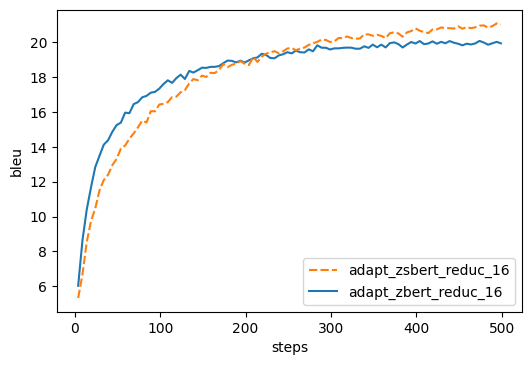
\includegraphics[width=0.95\textwidth]{img/zbert_vs_zsbert.png}}
    \centering
    \caption{Comparison adapters performance in \texttt{zsbert} and \texttt{zbert}. Both are using reduction ratio 16 and the adapters are placed on encoder and decoder.}
    \label{img:zbert_vs_zsbert}
\end{figure}

We see similar behaviour as we see on \texttt{zbert} experiments in regards to the position of the adapters. In \cref{img:zsbert_pos}, the benefit of incorporating adapters on the encoder side is also apparent and outperforms the decoder counterpart. We can also see a similar behaviour where eventually, the model's performance with adapters on the encoder outperforms the model with adapters on both sides. Furthermore, we also see similar behaviour as in \texttt{zbert} for models with adapters where the performance is very close to the baseline and not improving as much as the encoder side. We hypothesize the same reason as we have stated in \texttt{zbert} could apply in \texttt{zsbert} as well. Essentially, we need to modify the representation on the encoder side in order to achieve better performance.
